\documentclass[
  shownotes,
  xcolor={svgnames},
  hyperref={colorlinks,citecolor=DarkBlue,linkcolor=DarkRed,urlcolor=DarkBlue}
  ]{beamer}
\usepackage{animate}
\usepackage{amsmath}
\usepackage{amsfonts}
\usepackage{amssymb}
\usepackage{pifont}
\usepackage{mathpazo}
%\usepackage{xcolor}
\usepackage{multimedia}
\usepackage{fancybox}
\usepackage[para]{threeparttable}
\usepackage{multirow}
\setcounter{MaxMatrixCols}{30}
\usepackage{subcaption}
\usepackage{graphicx}
\usepackage{lscape}
\usepackage[compatibility=false,font=small]{caption}
\usepackage{booktabs}
\usepackage{ragged2e}
\usepackage{chronosys}
\usepackage{appendixnumberbeamer}
\usepackage{animate}
\setbeamertemplate{caption}[numbered]
\usepackage{color}
%\usepackage{times}
\usepackage{tikz}
\usepackage{comment} %to comment
%% BibTeX settings
\usepackage{natbib}
\bibliographystyle{apalike}
\bibpunct{(}{)}{,}{a}{,}{,}
\setbeamertemplate{bibliography item}{[\theenumiv]}

% Defines columns for bespoke tables
\usepackage{array}
\newcolumntype{L}[1]{>{\raggedright\let\newline\\\arraybackslash\hspace{0pt}}m{#1}}
\newcolumntype{C}[1]{>{\centering\let\newline\\\arraybackslash\hspace{0pt}}m{#1}}
\newcolumntype{R}[1]{>{\raggedleft\let\newline\\\arraybackslash\hspace{0pt}}m{#1}}


\usepackage{xfrac}


\usepackage{multicol}
\setlength{\columnsep}{0.5cm}

% Theme and colors
\usetheme{Boadilla}

% I use steel blue and a custom color palette. This defines it.
\definecolor{andesred}{HTML}{af2433}

% Other options
\providecommand{\U}[1]{\protect\rule{.1in}{.1in}}
\usefonttheme{serif}
\setbeamertemplate{itemize items}[default]
\setbeamertemplate{enumerate items}[square]
\setbeamertemplate{section in toc}[circle]

\makeatletter

\definecolor{mybackground}{HTML}{82CAFA}
\definecolor{myforeground}{HTML}{0000A0}

\setbeamercolor{normal text}{fg=black,bg=white}
\setbeamercolor{alerted text}{fg=red}
\setbeamercolor{example text}{fg=black}

\setbeamercolor{background canvas}{fg=myforeground, bg=white}
\setbeamercolor{background}{fg=myforeground, bg=mybackground}

\setbeamercolor{palette primary}{fg=black, bg=gray!30!white}
\setbeamercolor{palette secondary}{fg=black, bg=gray!20!white}
\setbeamercolor{palette tertiary}{fg=white, bg=andesred}

\setbeamercolor{frametitle}{fg=andesred}
\setbeamercolor{title}{fg=andesred}
\setbeamercolor{block title}{fg=andesred}
\setbeamercolor{itemize item}{fg=andesred}
\setbeamercolor{itemize subitem}{fg=andesred}
\setbeamercolor{itemize subsubitem}{fg=andesred}
\setbeamercolor{enumerate item}{fg=andesred}
\setbeamercolor{item projected}{bg=gray!30!white,fg=andesred}
\setbeamercolor{enumerate subitem}{fg=andesred}
\setbeamercolor{section number projected}{bg=gray!30!white,fg=andesred}
\setbeamercolor{section in toc}{fg=andesred}
\setbeamercolor{caption name}{fg=andesred}
\setbeamercolor{button}{bg=gray!30!white,fg=andesred}


\usepackage{fancyvrb}
\newcommand{\VerbBar}{|}
\newcommand{\VERB}{\Verb[commandchars=\\\{\}]}
\DefineVerbatimEnvironment{Highlighting}{Verbatim}{commandchars=\\\{\}}
% Add ',fontsize=\small' for more characters per line
\usepackage{framed}
\definecolor{shadecolor}{RGB}{248,248,248}
\newenvironment{Shaded}{\begin{snugshade}}{\end{snugshade}}
\newcommand{\AlertTok}[1]{\textcolor[rgb]{0.94,0.16,0.16}{#1}}
\newcommand{\AnnotationTok}[1]{\textcolor[rgb]{0.56,0.35,0.01}{\textbf{\textit{#1}}}}
\newcommand{\AttributeTok}[1]{\textcolor[rgb]{0.77,0.63,0.00}{#1}}
\newcommand{\BaseNTok}[1]{\textcolor[rgb]{0.00,0.00,0.81}{#1}}
\newcommand{\BuiltInTok}[1]{#1}
\newcommand{\CharTok}[1]{\textcolor[rgb]{0.31,0.60,0.02}{#1}}
\newcommand{\CommentTok}[1]{\textcolor[rgb]{0.56,0.35,0.01}{\textit{#1}}}
\newcommand{\CommentVarTok}[1]{\textcolor[rgb]{0.56,0.35,0.01}{\textbf{\textit{#1}}}}
\newcommand{\ConstantTok}[1]{\textcolor[rgb]{0.00,0.00,0.00}{#1}}
\newcommand{\ControlFlowTok}[1]{\textcolor[rgb]{0.13,0.29,0.53}{\textbf{#1}}}
\newcommand{\DataTypeTok}[1]{\textcolor[rgb]{0.13,0.29,0.53}{#1}}
\newcommand{\DecValTok}[1]{\textcolor[rgb]{0.00,0.00,0.81}{#1}}
\newcommand{\DocumentationTok}[1]{\textcolor[rgb]{0.56,0.35,0.01}{\textbf{\textit{#1}}}}
\newcommand{\ErrorTok}[1]{\textcolor[rgb]{0.64,0.00,0.00}{\textbf{#1}}}
\newcommand{\ExtensionTok}[1]{#1}
\newcommand{\FloatTok}[1]{\textcolor[rgb]{0.00,0.00,0.81}{#1}}
\newcommand{\FunctionTok}[1]{\textcolor[rgb]{0.00,0.00,0.00}{#1}}
\newcommand{\ImportTok}[1]{#1}
\newcommand{\InformationTok}[1]{\textcolor[rgb]{0.56,0.35,0.01}{\textbf{\textit{#1}}}}
\newcommand{\KeywordTok}[1]{\textcolor[rgb]{0.13,0.29,0.53}{\textbf{#1}}}
\newcommand{\NormalTok}[1]{#1}
\newcommand{\OperatorTok}[1]{\textcolor[rgb]{0.81,0.36,0.00}{\textbf{#1}}}
\newcommand{\OtherTok}[1]{\textcolor[rgb]{0.56,0.35,0.01}{#1}}
\newcommand{\PreprocessorTok}[1]{\textcolor[rgb]{0.56,0.35,0.01}{\textit{#1}}}
\newcommand{\RegionMarkerTok}[1]{#1}
\newcommand{\SpecialCharTok}[1]{\textcolor[rgb]{0.00,0.00,0.00}{#1}}
\newcommand{\SpecialStringTok}[1]{\textcolor[rgb]{0.31,0.60,0.02}{#1}}
\newcommand{\StringTok}[1]{\textcolor[rgb]{0.31,0.60,0.02}{#1}}
\newcommand{\VariableTok}[1]{\textcolor[rgb]{0.00,0.00,0.00}{#1}}
\newcommand{\VerbatimStringTok}[1]{\textcolor[rgb]{0.31,0.60,0.02}{#1}}
\newcommand{\WarningTok}[1]{\textcolor[rgb]{0.56,0.35,0.01}{\textbf{\textit{#1}}}}
\usepackage{graphicx}
\makeatletter

\makeatother






%%%%%%%%%%%%%%% BEGINS DOCUMENT %%%%%%%%%%%%%%%%%%

\begin{document}

\title[Lecture 6]{Lecture 6: \\ OLS Computation \\ Intro To Scraping}
\subtitle{Big Data and Machine Learning for Applied Economics \\ Econ 4676}
\date{\today}

\author[Sarmiento-Barbieri]{Ignacio Sarmiento-Barbieri}
\institute[Uniandes]{Universidad de los Andes}


\begin{frame}[noframenumbering]
\maketitle
\end{frame}

%%%%%%%%%%%%%%%%%%%%%%%%%%%%%%%%%%%



%----------------------------------------------------------------------%

\begin{frame}
\frametitle{Recap}


  \begin{itemize} 
    \item What is Big Data?
    \medskip
    \item Quick Review of Statistical Properties
    \medskip
    \item Numerical Properties
    \medskip
    \item FWL
    \begin{itemize}
    \item Fixed Effects
    \item Leverage
    \item Goodness of Fit
  \end{itemize}
  \end{itemize}
  
\end{frame}

%----------------------------------------------------------------------%

\begin{frame}
\frametitle{Agenda}

\tableofcontents


\end{frame}



%----------------------------------------------------------------------%
\section{Computation}
%----------------------------------------------------------------------%


%----------------------------------------------------------------------%
\subsection{Traditional Computation}
%----------------------------------------------------------------------%
\begin{frame}[fragile]
\frametitle{Motivation}

\begin{itemize}
\item OLS workhorse

\begin{align}
\hat \beta=(X'X)^{-1}X'y
\end{align}

\item Involves inverting a $k\times k$ matrix $X'X$
\item requires allocating $O (nk+k^2)$ if n is "big" we cannot store this in memory

\end{itemize}

Solving directly


\begin{Shaded}
%\begin{Highlighting}[]
\begin{verbatim}
beta<-solve(t(X)%*%X)%*%t(X)%*%y
\end{verbatim}
%\end{Highlighting}
\end{Shaded}


may not be the smartest move

    
  
\end{frame}

%----------------------------------------------------------------------%
\begin{frame}[fragile]
\frametitle{\texttt{QR} decomposition:}
Most software use a \texttt{QR} decomposition:
 
 \begin{Shaded}
{\bf Theorem}
If $A\in\mathbb{R}^{n\times k}$ then there exists an orthogonal $Q\in \mathbb{R}^{n\times n}$ and an upper triangular $R\in \mathbb{R}^{n\times k}$ so that $A=QR$
\end{Shaded}

\begin{itemize}
  \footnotesize
  \item Orthogonal Matrices: 
  \begin{itemize}
    \tiny
  \item Def: $Q'Q=QQ'=I$ and $Q'=Q^{-1}$
  \item Prop: product of orthogonal is orthogonal, e.g $A'A=I$ and $B'B=I$ then $(AB)'(AB)=B'(A'A)B=B'B=I$
  \end{itemize}
  \item {\bf (Thin QR)} If $A\in\mathbb{R}^{n\times k}$   has full column rank then $A=Q_1R_1$ the QR factorization is unique, where $Q_1 \in\mathbb{R}^{n\times k}$ and $R$ is upper triangular with  positive diagonal entries
\end{itemize}

Can use it these to get $\hat \beta$

\footnotesize
\begin{align}
  (X'X) \hat \beta &=  X'y  \\
  (R'Q'QR) \hat \beta &=  R'Q'y  \\
  (R'R) \hat \beta &=  R'Q'y  \\
  R \hat \beta &=  Q'y  
\end{align}
Solve by back substitution

\end{frame}

%----------------------------------------------------------------------%
\begin{frame}[fragile]
\frametitle{\texttt{QR} decomposition:}

\footnotesize
\begin{align}
X=\left[\begin{array}{cc}
1 & 2\\
1 & 2\\
1 & 3
\end{array}\right]\,\,
 y=\left(\begin{array}{c}
1\\
4\\
2
\end{array}\right)
\end{align}
1. QR factorization  X=QR
\begin{align}
Q=\left[\begin{array}{cc}
-0.57 & -0.41 \\
-0.57 & -0.41 \\
-0.57 & 0.82
\end{array}\right]\,\,
R=\left[\begin{array}{cc}
-1.73 & -4.04 \\
1 & 0.81 
\end{array}\right]
\end{align}
2. Calculate $Q'y=[-4.04,-0.41]'$

3. Solve

\begin{align}
\left[\begin{array}{cc}
-1.73 & -4.04 \\
1 & 0.81 
\end{array}\right]\left[\begin{array}{c}
\beta_1 \\
\beta_2 
\end{array}\right]=\left[\begin{array}{c}
-4.04 \\
-0.41
\end{array}\right]
\end{align}

Solution is $(3.5, -0.5)$
\end{frame}

%----------------------------------------------------------------------%
\begin{frame}[fragile]
\frametitle{\texttt{QR} decomposition:}
This is actually what \texttt{R} does under the hood


\begin{figure}[H] \centering
  \centering
  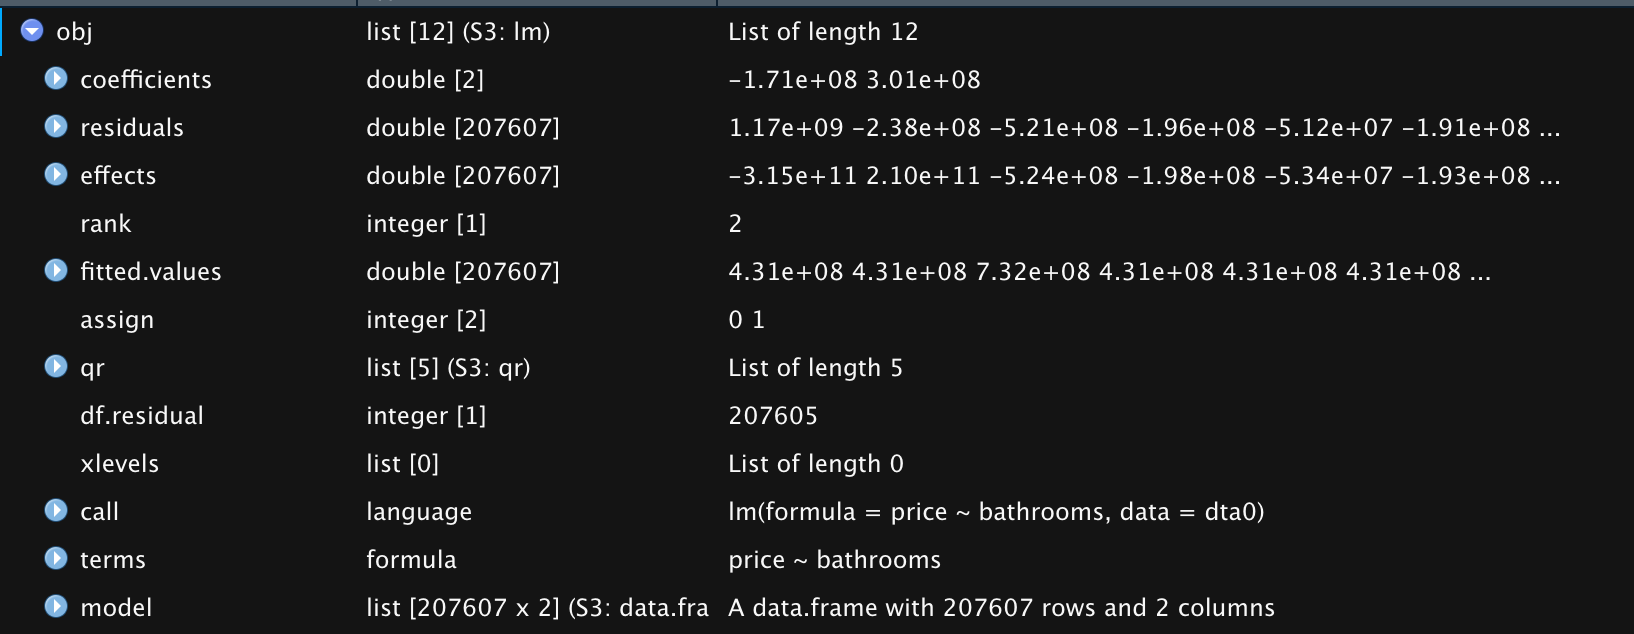
\includegraphics[scale=0.45]{figures/lm_object.png}
  \\
  \tiny 
\end{figure}


Note that \texttt{R's} \texttt{lm} also returns many objects that have the same size as X and Y

\end{frame}

%----------------------------------------------------------------------%
%----------------------------------------------------------------------%
\subsection{Parallel vs Distributed}
%----------------------------------------------------------------------%
\begin{frame}
\frametitle{Parallel vs Distributed}

\begin{itemize}
\item An algorithm is parallel if it does many computations at once. 
\begin{itemize}
  \item It needs to see all of the data
\end{itemize}
\medskip
\item It is distributed if you can work with subsets of data
\begin{itemize}
  \item \texttt{Stata-mp} is parallel. (license charges by core)
  \item \texttt{R} and \texttt{Python} can be parallel {\bf and} distributed
  \end{itemize}
\end{itemize}


\begin{figure}[H] \centering
  \centering
  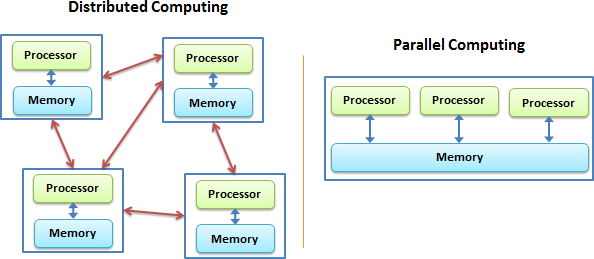
\includegraphics[scale=0.65]{figures/distributed_parallel.png}
  \\
  \tiny \url{https://tinyurl.com/y3nzvkwh}
\end{figure}


\end{frame}

%----------------------------------------------------------------------%
\begin{frame}
\frametitle{Map Reduce}

\begin{itemize}
  \item  Original Paper {\it MapReduce: Simplified data processing on large clusters (2004) Dean and Ghemawat}
  \medskip 
  \item It is of the most popular frameworks 
  \medskip
  \item Basic Idea:

  
\begin{enumerate}
  \item You need to be able to specify a key that indexes subgroups of data that can be analyzed in isolation.
  \item Map: Calculate and sort relevant statistics by key
  \item Partition and pipe the outcome of map so that outcomes with the same key end up on the same machine
  \item Reduce: Apply a summarization operation within the subgroup defined by each key.
\end{enumerate}
\end{itemize}



   
\end{frame}

%----------------------------------------------------------------------%
\begin{frame}
\frametitle{Example: Mean by groups}



\begin{figure}[H] \centering
  \centering
  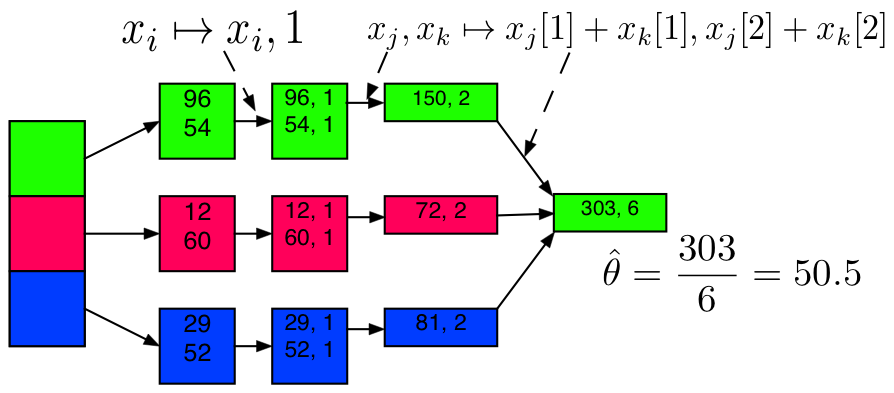
\includegraphics[scale=0.65]{figures/sketch_model_example.png}
  \\
  \tiny \url{https://datascienceguide.github.io/map-reduce}
\end{figure}

\end{frame}

%----------------------------------------------------------------------%
\begin{frame}[fragile]
\frametitle{\texttt{QR} decomposition for block matrices}
\tiny 
Idea on how to distribute OLS (Constantine \& Gleich, 2011)


\begin{align}
X_{8n\times k}=\left[\begin{array}{c}
X_{2n\times k}^{1}\\
X_{2n\times k}^{2}\\
X_{2n\times k}^{3}\\
X_{2n\times k}^{4}
\end{array}\right]
\end{align}


QR to each block

\begin{align}
X_{8n\times k}=\underset{8n\times4k}{\underbrace{\left[\begin{array}{cccc}
Q_{2n\times k}^{1}\\
 & Q_{2n\times k}^{2}\\
 &  & Q_{2n\times k}^{3}\\
 &  &  & Q_{2n\times k}^{4}
\end{array}\right]}}\underset{4k\times k}{\underbrace{\left[\begin{array}{c}
R_{k\times k}^{1}\\
R_{k\times k}^{2}\\
R_{k\times k}^{3}\\
R_{k\times k}^{4}
\end{array}\right]}}
\end{align}

\begin{align}
X_{8n\times k}=\underset{Q}{\underbrace{\underset{8n\times4k}{\underbrace{\left[\begin{array}{cccc}
Q_{2n\times k}^{1}\\
 & Q_{2n\times k}^{2}\\
 &  & Q_{2n\times k}^{3}\\
 &  &  & Q_{2n\times k}^{4}
\end{array}\right]}}\underset{4k\times k}{\underbrace{Q_{2}}}}}\underset{k\times k}{\underbrace{R_{2}}}
\end{align}

\end{frame}


%----------------------------------------------------------------------%
\begin{frame}
\frametitle{Spark}

\begin{itemize}
  \item  The tools facilitating distributed computing are rapidly improving. 
  \medskip
  \item One prominent system is Spark, that is quickly replacing MapReduce
  \medskip
  \item Seamlessly integration with \texttt{R} and \texttt{Python} and has it's own \texttt{MLlib}
  \medskip
  \begin{itemize}
   \item E.g. Spark uses distributed version of stochastic gradient descent to compute OLS  
    \end{itemize}       
    \item One of the key differences with MapReduce is how they load data 
    \begin{itemize}
     \item MapReduce has to read from and write to a disk
     \item Spark loads it  in-memory (can get 100x faster)
    \end{itemize}       

\end{itemize}    
  
\end{frame}


%----------------------------------------------------------------------%
\section{Web scraping}
%----------------------------------------------------------------------%
\begin{frame}
\frametitle{Motiviation Webscraping}



\begin{figure}[H] \centering
  \centering
  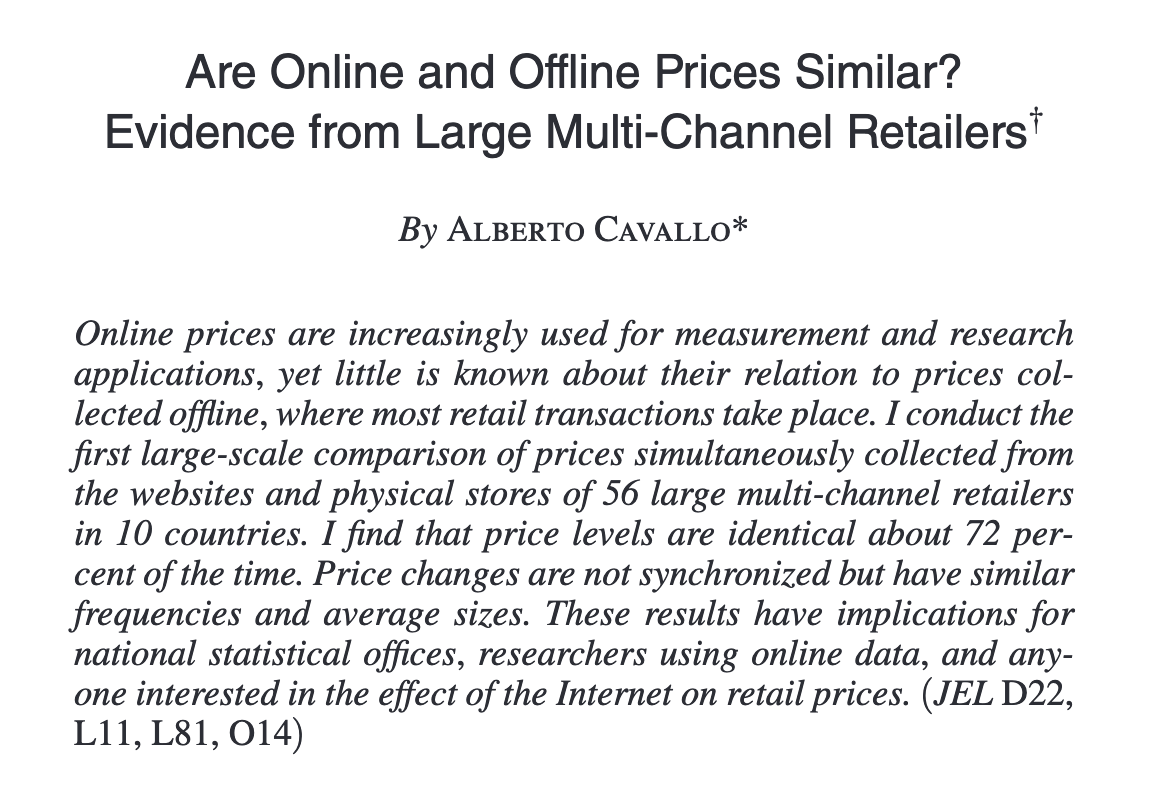
\includegraphics[scale=0.45]{figures/Cavallo_title}
  \\
  \tiny
\end{figure}
 

\end{frame}

%----------------------------------------------------------------------%
\begin{frame}
\frametitle{Motiviation Webscraping}



\begin{figure}[H] \centering
  \centering
  
\includegraphics[scale=0.25]{figures/Cunningham_title}
  \\
  \tiny
\end{figure}
 

\end{frame}

%----------------------------------------------------------------------%

\begin{frame}
\frametitle{Motiviation Webscraping}



\begin{figure}[H] \centering
  \centering
  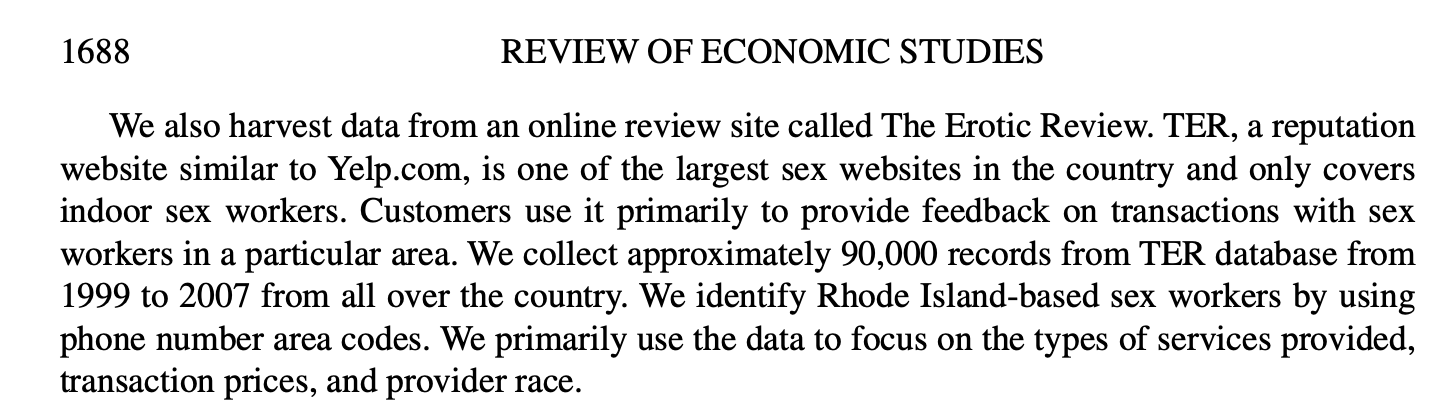
\includegraphics[scale=0.45]{figures/Cunningham_desc}
  \\
  \tiny
\end{figure}
 

\end{frame}


%----------------------------------------------------------------------%

\begin{frame}
\frametitle{Webscraping basics}

\begin{figure}[H] \centering
  \centering
  
\includegraphics[scale=0.75]{figures/webscrape_it.jpg}
  \\
  \tiny
\end{figure}

\end{frame}

%----------------------------------------------------------------------%
\begin{frame}
\frametitle{Webscraping basics}

\begin{itemize}
  \item How to get data, or "content", off the web and onto our computers.
  \bigskip
  \item If you see it in your browser it exists somewhere
  \bigskip
  \item To be ``successful'' one must have a working knowledge on:
  \begin{itemize}
  \item how web pages display content (Hyper Text Markup Language or HTML)
  \medskip
  \item where is the content ``located''


    \begin{enumerate}
    \item Server side
    \medskip
    \item Client side
    \medskip

    \end{enumerate}
    \item The good news is that both server-side and client-side websites allow for web scraping
   \end{itemize}
\end{itemize}





\end{frame}

%----------------------------------------------------------------------%
\begin{frame}
\frametitle{Caveat: ethical and legal limitations}

\begin{itemize}
\item Just because you *can* scrape it, doesn't mean you *should*. 
\medskip
\item Check \texttt{The Robots Exclusion Protocol} of a website, adding \texttt{``/robots.txt''} to the website's URL
\begin{enumerate}
  \item User-agent:  the type of robots to which the section applies
  \item Disallow:  directories/prefixes of the website not allowed to robots
  \item Allow:  sections of the website allowed to robots
\end{enumerate}
\medskip
\item \texttt{robots.txt} is de facto standard (see \url{http://www.robotstxt.org})
\medskip
\item Also always check the terms and conditions and what they say about scraping
\medskip
\item Remember the immortal words of uncle Ben: ``with great power comes great responsibility''

\end{itemize}


\end{frame}
%----------------------------------------------------------------------%
\begin{frame}
\frametitle{Server-side}

\begin{itemize}

\item The website is "static", all the info is located in the HTML code that the host server sends
\medskip
\begin{itemize}
  \item  E.g. Wikipedia tables are already populated with all of the information - tables, numbers, dates, etc. - that we see in our browser.
\end{itemize}
\bigskip
\item  Challenges: 
\medskip
\begin{itemize}
  \item Finding the correct path CSS (or Xpath) "selectors". 
  \item Navigating dynamic webpages (e.g. "Next page" and "Show More" tabs).
\end{itemize} 
 \end{itemize} 
\end{frame}


%----------------------------------------------------------------------%
\begin{frame}
\frametitle{Some useful tools}


\begin{itemize}
  \item CSS selectors:
  \begin{itemize}
   \item \href{https://selectorgadget.com/}{SelectorGadget} for Chrome
   \item \href{https://addons.mozilla.org/en-US/firefox/addon/scrapemate/}{ScrapeMate} for Firefox
   \item Inspect Element

  \end{itemize}
  \item Browsers: anything but explorer
\end{itemize}


\begin{figure}[H] \centering
  \centering
  
\includegraphics[scale=0.45]{figures/explorer_crying.jpg}
  \\
  \tiny
\end{figure}
 

\end{frame}

%----------------------------------------------------------------------%
\begin{frame}
\frametitle{Client-side}  
\begin{itemize}

\item The website contains an empty template of HTML and CSS. 
\begin{itemize}
  \item E.g. It might contain a "skeleton" table without any values.
  \end{itemize} 
  \medskip
\item However, when we actually visit the page URL, our browser sends a *request* to the host server.
\medskip
\item If request is valid, then the server sends a response script, which our browser executes and uses to populate the HTML template with the specific information that we want.
\medskip
\item Challenges: Finding the "API endpoints" can be tricky, since these are sometimes hidden from view.

\end{itemize} 


\end{frame}

%----------------------------------------------------------------------%

\begin{frame}
\frametitle{Demo}

\begin{figure}[H] \centering
  \centering
  
\includegraphics[scale=0.25]{figures/baticomputer_meme.jpg}
  \\
  \tiny photo from \url{https://www.dailydot.com/parsec/batman-1966-labels-tumblr-twitter-vine/}
\end{figure}

\end{frame}

%----------------------------------------------------------------------%

\begin{frame}
\frametitle{Review \& Next Steps}
  
  \begin{itemize} 
    \item Computation
    \item QR decomposition
    \item MapReduce and Spark
    \item Demo \texttt{Scraping}
    \item Message: web scraping involves as much art as it does science
  \bigskip  

  
  \item  {\bf Next Class:} MLE, Bayesian Stats.
  \bigskip
  \item Questions? Questions about software? 
  
  \end{itemize}


\end{frame}


%----------------------------------------------------------------------%

\section{Further Readings}
%----------------------------------------------------------------------%
\begin{frame}
\frametitle{Further Readings}
\footnotesize
\begin{itemize}
  
  \item Constantine, P. G., \& Gleich, D. F. (2011, June). Tall and skinny QR factorizations in MapReduce architectures. In Proceedings of the second international workshop on MapReduce and its applications (pp. 43-50).
  \medskip
  \item Dean, J., \& Ghemawat, S. (2004). MapReduce: Simplified data processing on large clusters.
  \medskip
  \item Van Loan, C. F., Golub, G. H. (2012). Matrix Computations. United States: Johns Hopkins University Press.
  \medskip
  \item \texttt{Webscraping} tutorial from  \href{https://grantmcdermott.com/}{Prof.~Grant McDermott}.
  \medskip
  \item \href{https://www.sas.upenn.edu/~jesusfv/Lecture_HPC_10_Web_Scrapping.pdf}{Web Scrapping slides} from Fernandez Villaverde J., Guerrón P. \& Zarruk Valencia, D. 
  \medskip
  \item Wickham, H., \& Wickham, M. H. (2016). Package ‘rvest’. \url{https://cran.r-project.org/web/packages/rvest/rvest.pdf}.
  
\end{itemize}

\end{frame}


\end{document}


